%%%%%%%%%%%%%%%%%%%%%%%%%%%%%%%%%%%%%%%%%%%%%%%%%%%%%%%%%%%%%%%%%%%%%%%%%%%%%
%%%
%%% File: utthesis2.doc, version 2.0jab, February 2002
%%%
%%% Based on: utthesis.doc, version 2.0, January 1995
%%% =============================================
%%% Copyright (c) 1995 by Dinesh Das.  All rights reserved.
%%% This file is free and can be modified or distributed as long as
%%% you meet the following conditions:
%%%
%%% (1) This copyright notice is kept intact on all modified copies.
%%% (2) If you modify this file, you MUST NOT use the original file name.
%%%
%%% This file contains a template that can be used with the package
%%% utthesis.sty and LaTeX2e to produce a thesis that meets the requirements
%%% of the Graduate School of The University of Texas at Austin.
%%%
%%% All of the commands defined by utthesis.sty have default values (see
%%% the file utthesis.sty for these values).  Thus, theoretically, you
%%% don't need to define values for any of them; you can run this file
%%% through LaTeX2e and produce an acceptable thesis, without any text.
%%% However, you probably want to set at least some of the macros (like
%%% \thesisauthor).  In that case, replace "..." with appropriate values,
%%% and uncomment the line (by removing the leading %'s).
%%%
%%%%%%%%%%%%%%%%%%%%%%%%%%%%%%%%%%%%%%%%%%%%%%%%%%%%%%%%%%%%%%%%%%%%%%%%%%%%%

%%%%%%%%%%%%%%%%%%%%%%%%%%%%%%%%%%%%%%%%%%%%%%%%%%%%%%%%%%%%%%%%%%%%%%%%%%%%%
%%%
%%
%% This file, and the corresponding tcdthesis.sty the accompanied it, have
%% been modified for the M.Sc. styles used in Trinity College, Dublin
%%
%%
%%%%%%%%%%%%%%%%%%%%%%%%%%%%%%%%%%%%%%%%%%%%%%%%%%%%%%%%%%%%%%%%%%%%%%%%%%%%%
\documentclass[a4paper, 12pt, oneside]{report}         %% LaTeX2e document.
\usepackage {testthesis}              %% Preamble.

\mastersthesis                     %% Uncomment one of these; if you don't
% \phdthesis                         %% use either, the default is \phdthesis.

\thesisdraft                       %% Uncomment this if you want a draft
                                     %% version; this will print a timestamp
                                     %% on each page of your thesis.

\leftchapter                       %% Uncomment one of these if you want
%\centerchapter                      %% left-justified, centered or
% \rightchapter                      %% right-justified chapter headings.
                                     %% Chapter headings includes the
                                     %% Contents, Acknowledgments, Lists
                                     %% of Tables and Figures and the Vita.
                                     %% The default is \centerchapter.

% \singlespace                       %% Uncomment one of these if you want
\oneandhalfspace                   %% single-spacing, space-and-a-half
% \doublespace                       %% or double-spacing; the default is
                                     %% \oneandhalfspace, which is the
                                     %% minimum spacing accepted by the
                                     %% Graduate School.

\renewcommand{\thesisauthor}{...}            %% Your official TCD name.
\renewcommand{\thesismonth}{...}                  %% Your month of graduation.
\renewcommand{\thesisyear}{...}                      %% Your year of graduation.
\renewcommand{\thesistitle}{...}            %% The title of your thesis; use mixed-case.
\renewcommand{\thesisauthorpreviousdegrees}{...}  %% Your previous degrees, abbreviated; separate multiple degrees by commas.
\renewcommand{\thesissupervisor}{...}      %% Your thesis supervisor; use mixed-case and don't use any titles or degrees.
% \renewcommand{\thesiscosupervisor}{}                %% Your PhD. thesis co-supervisor; if any.

% \renewcommand{\thesiscommitteemembera}{}
% \renewcommand{\thesiscommitteememberb}{}
% \renewcommand{\thesiscommitteememberc}{}
% \renewcommand{\thesiscommitteememberd}{}
% \renewcommand{\thesiscommitteemembere}{}
% \renewcommand{\thesiscommitteememberf}{}
% \renewcommand{\thesiscommitteememberg}{}
% \renewcommand{\thesiscommitteememberh}{}
% \renewcommand{\thesiscommitteememberi}{}


\renewcommand{\thesisauthoraddress}{...}

\renewcommand{\thesisdedication}{...}     %% Your dedication, if you have one; use "\\" for linebreaks.


%%%%%%%%%%%%%%%%%%%%%%%%%%%%%%%%%%%%%%%%%%%%%%%%%%%%%%%%%%%%%%%%%%%%%%%%%%%%%
%%%
%%% The following commands are all optional, but useful if your requirements
%%% are different from the default values in tcdthesis.sty.  To use them,
%%% simply uncomment (remove the leading %) the line(s).

\renewcommand{\thesisdegree}{Master of Science in Computer Science}  
                                     %% default is "DOCTOR OF PHILOSOPHY"
                                     %% for \phdthesis or "MASTER OF ARTS"
                                     %% for \mastersthesis.  Provide the
                                     %% correct FULL OFFICIAL name of
                                     %% the degree.
\renewcommand{\thesisdegreestream}{ (Data Science)}
                                     %% Default is empty. This is used on
                                     %% the title page of the thesis.

\renewcommand{\thesisdegreeabbreviation}{M.Sc.}
                                     %% Use this if you also use the above
                                     %% command; provide the OFFICIAL
                                     %% abbreviation of your thesis degree.
\renewcommand{\thesistype}{Dissertation}    %% Use this ONLY if your thesis type
                                     %% is NOT "Thesis" for \phdthesis
                                     %% or \mastersthesis.
                                     %% Provide the OFFICIAL type of the
                                     %% thesis; use mixed-case.

% \renewcommand{\thesistypist}{...}  %% Use this to specify the name of
                                     %% the thesis typist if it is anything
                                     %% other than "the author".

%%%
%%%%%%%%%%%%%%%%%%%%%%%%%%%%%%%%%%%%%%%%%%%%%%%%%%%%%%%%%%%%%%%%%%%%%%%%%%%%%



\begin{document}                                  %% BEGIN THE DOCUMENT

\thesistitlepage                                  %% Generate the title page.

\thesisdeclarationpage                %% Generate the declaration page.

\thesispermissionpage                 %% Generate the copyright permission page

%\thesisdedicationpage                             %% Generate the dedication page.

\begin{thesisacknowledgments}                     %% Use this to write your
...ACKNOWLEDGMENTS...                          %% acknowledgments; it can be anything
\end{thesisacknowledgments}                       %% allowed in LaTeX2e par-mode.

\begin{thesisabstract}                          %% the abstract for your thesis
...ABSTRACT...
\end{thesisabstract}

\begin{thesissummary}                           %% The summary page for your thesis
...SUMMARY...	
\end{thesissummary}


\tableofcontents                                  %% Generate table of contents.
\listoftables                                     %% Uncomment this to generate list of tables.
\listoffigures                                    %% Uncomment this to generate list of figures.

%%
%% Include thesis chapters here...
%%
  


\chapter{State Of The Art}
\section{Multi Protocol Label Switching (MPLS)}

In MPLS Networks, Packets are forwarded using the 20 Byte Labels unlike the 32 bit IP Address. In order to understand the working of MPLS and its advantages over conventional IP Network, we must understand how the traditional IP traffic processed. 

\subsection{IP Routing}

IP routing\cite{2008} is the process of sending packets from one L3 host to another. The hosts can be in same or different networks and the networks are identified using the IP Addresses. Each packet will have a field for source address and destination address and the packets are forwarded based on the destination address. All the IP Networking devices will maintain a routing table. The devices can be a host machine or a router. The routing table consists of an address field where we can see a 32 bit address and an interface field where we can see a physical or logical interface corresponding to the address. 

\begin{figure}
       \centering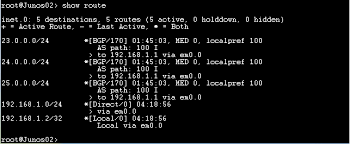
\includegraphics[width=\textwidth]{Final/routing table.png}
       \caption{Sample routing table}
       \label{fig:compbest}
\end{figure}

The figure 1.1 is a sample of routing table from a Juniper router. We can see the networks and the corresponding exit interfaces. Theses routing tables are created and maintained by different routing protocols and each routing protocol have its own mechanisms of finding the best route to the destination. OSPF, RIP and BGP are the well-known routing protocols\cite{2005}.

\subsection{MPLS Switching} 

Multi-protocol label switching (MPLS)\cite{farrel_2004}, is a technique that uses 20-bit labels instead of 32-bit IP Address for sending packet from one MPLS router to another. The Labels are pre populated using different protocols such as Label Distribution Protocol (LDP), Resource Reservation Protocol (RSVP) or Multiprotocol BGP (MP BGP). The packet switching is happening at 2.5 header of the OSI reference model and hence it's called switching. As MPLS need the help of other protocols to create the labels, the name multi-protocol labelled switching  

 \begin{figure}
       \centering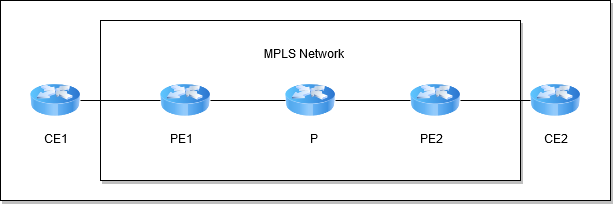
\includegraphics[width=\textwidth]{Final/MPLS Network.png}
       \caption{MPLS Network}
       \label{fig:compbest}
\end{figure}

In the Figure 1.2 the CE1 is a L3 router which operates exclusively on IP address and PE1 is called provider edge router which will operate on both IP address and labels. P is provider router which works exclusively on labels. The incoming packets from CE1 in PE1 taken to a class called Forward equivalence class which assign a label corresponding to the destination IP address. The PE1 then forward the packet to P router which will pop the existing label and add its label corresponding to the destination and finally PE2 will pop the MPLS header from the packet and forward the packet to CE2 using IP routing table. 



 

 \begin{figure}
       \centering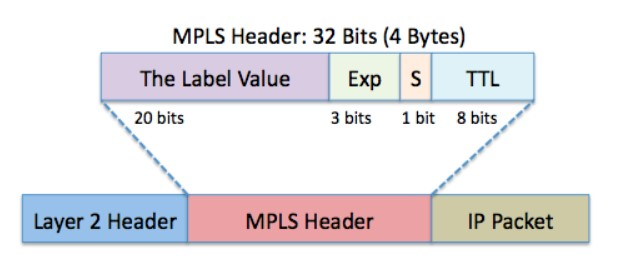
\includegraphics[width=\textwidth]{Final/MPLS Header.jpg}
       \caption{MPLS Header}
       \label{fig:compbest}
\end{figure}


MPLS header gets in between the Ethernet header and the IP Header. The header is 4 bytes in size. The first 20 bits are for the labels, the next 3 bits are for class of service and the next 1 bit for the bottom of stack flag which basically say where the label is positioned. The last 8 bits are for the TTL (time to live). 

\section{Security Requirements in MPLS}

As we know that MPLS is a widely used technology by Service provider to provide VPN Services, the expectation from the VPN Customers and the Service provider is that MPLS Should inherently possess basic security requirements\cite{2010} by its architecture. In this section we can see the basic security requirements of an MPLS Network\cite{davie_farrel_2008}.

\subsection{Address Space Separation}


The expectation is that a packet destined to a host with a particular address in a VPN shouldn't’t reach another VPN or the core. MPLS assume unique address space between 2 non intersecting VPNs and the address space between VPNs should be absolutely independent. This is a basic assumption of address space in MPLS VPNs. In another words the address space in a VPN is very private to it and the same address may can be used in different VPNs for its local connectivity. The routing between 2 VPNs or the VPN and the MPLS core should be independent. Adding a 64-bit RD (Route Distinguisher) by the MPLS core to each IPv4 route will make the VPN unique with the address and unique to the core. The exception is that The IP address of the link between the Provider Edge (PE) and the Customer Edge (CE) router are connected with must be unique. Every PE router is maintaining a VRF table (Virtual Router Forwarding) for each VPNs it connected with. This VRF tables separates the routing between the VPNs. In MPBGP (A signalling protocol), between the core to the other PE routers, the separation is maintained by unique VPN identifiers (VPN ID). This Information is redistributed to all the PE routers and available to all the PEs. So, unless configured to, a packet to host through a VPN cannot reach another VPN.

\subsection{Hiding the MPLS Core from outside}


The Network provider usually hide the internal structure of the MPLS core from outside. In another word, a traceroute should not detail the MPLS Core routers and its addresses. If the internal details of the network are visible to an attacker, its easy to trigger a DOS (Denial-of-service) attack. The network detailing should be hidden even to the VPN Customers and Users. A simple continues ping to any of the PE or P routers in the MPLS core can make the router busy and lead to denial of services.
\subsection{Resistance to attacks}

The Network provider usually hide the internal structure of the MPLS core from outside. In another word. It is easy to trigger a DOS Attack to any exposed resource either by abusing the underlying Routing protocol or by abusing the Signalling protocol (example: attack LDP). This can make instabilities in the Network. 3 Solutions are possible in this case. 1 s isolate the core to the maximum from outside. 2nd is use various packet filters such as ACLs and filter unwanted traffic incoming from outside to the core. 3rd is use the authentication mechanisms provided by the routing protocols and signalling protocols (MD5 Authentication). Out of all these the strongest solution is the isolation of the MPLS Core. The Link connecting the CE and PE should be protected securely.
\subsection{Label spoofing}


As we already discussed that, the packets in MPLS Network is transmitted based on the labels and the PE router maintain an FEC and assign a label to the incoming packet. The design of MPLS is in such a way that the PE cannot accept a pre labelled packet. If an attacker can label an IP packet with a label, the PE cannot accept that, and it can lead to packet drop. So, protecting the packet from the data path of the CE router or even outside is very important. The result of label spoofing within the MPLS core can forward the packet to the convenience of the attacker. Hence protecting the packets from label spoofing Is very important in MPLS.

\section{Possible attacks in MPLS}


MPLS can be attacked in many ways\cite{grayson_guernsey_butts_spainhower_shenoi_2009}. There are tools available which can target various signalling protocols by sending dummy messages to initiate a session, keep the session open or close the session. Loki is one such tool which can use to attack MPLS. It can capture the packets, inject packets, firewall the packets. Let us see some attacks Loki can make in the MPLS Network. In this section, we will attempt to list the different safety assaults that are susceptible to the MPLS network. Security attacks were divided into four kinds: Data Plane Attacks, Control Plane Attacks, MPLS Network Operational and Management Attacks, and Insider Attacks.

\subsection{Attacks on the Data Plane}

Attacks aimed mainly at User or Service Provider data are categorized into data-plane security attacks. These attacks are either aimed at manipulating the data flowing through the MPLS network, removing the data flowing through the MPLS network, injecting malicious data or simply observing maliciously unauthorized data. 

\subsubsection{Taking the MPLS traffic outside the core} 

If an attacker has access to any core device, he can relabel or encapsulate an udp header with a destination address which attacker desired to send. Thus, the attacker can read or access the data from attacker's convenience. In order to do this, the attacker should be aware of the labels used in the traffic. Service providers usually hide the internal architecture of the MPLS core, but still it's not 100 percent safe. 

 
\subsubsection{Modify the Data Traffic}

Manipulating or changing the header fields of the packets can cause severe damage to MPLS Network. This is only possible when the MPLS Internals are exposed to the attacker. Getting the access of the MPLS core is however not easy since service providers usually hide the core from outside. Service providers use firewalls and other filters in their core to filter and block illegitimate packets and accesses. But once the attacker somehow managed to gain the core access, He/ She can make sever damage to the Networks. 

Listed few of the attacks which is possible by packet manipulations, they are: 

\subsubsection{Modify the routes}
 

Attacker can manipulate the network field of the packets the CE router can route the packets to a different destination out of the MPLS Cloud. Attacker can change the L3 field, Labels or encapsulate an UDP Header with completely different Network information. If the attacker gain access to packets part of financial transactions, we can imagine the damage. Rerouting of traffic can take one customers traffic to another customers network. \\

    Path Switching:   Generally, all MPLS packets flow through a Label switched path (LSP) assigned by the service provider. These paths are basically allocated by the service provider based on the labels associated to the packets. Labels are assigned by various parameters such as destination prefix or intended quality of service. For example, if Video streaming packets required a high bandwidth link, then the label will be of the LSP with higher throughput. If an attacker know the particular Label associated to the best LSP, he can label his local traffic such as online gaming traffic and gain best quality of service at the same time the genuine traffic which is expected good quality of service can get dropped. \\
    
    Destination Switching: This can be done in different ways. 1 is by changing the labels , 2nd by changing the destination IP address. Attacker can take the packets to any destination he/she desired and conduct malicious operations. \\
    
    Brute-Force Label Prediction: If an attacker know the destination address, then he/she can inject traffic with some random labels to MPLS networks. Attacker can injects packets by changing labels each time till get a reply from the destination and by doing this the attacker deduce the LSP. Once knew the label information of the LSP, he can use this for malicious operations.\\
    
    
    Address Messages Modification: This is very similar to Label modification. If an attacker gained access to the Customer edge router, he can manipulate the destination address field of the packet and the Provider edge router will take the packet to a Forward Equivalence Class for allocating a label. Suppose the FEC have no information or class for the destination address marked in the packet by attacker, might lead to create a New LSP and send the packets through a compromised link.\\

    Label Edge Router (LER) label Modification:  Customer edge routers are the routers which assign labels to the packets very first time in the MPLS Network and the core routers do the packet forwarding based on the labels PE assigned. If an attacker gained access to the PE router, he can pop the label which PE assigned and push a new label. The Provider router will have to choose an LSP according to the incoming label and if there is no LSP for the incoming label, then this might lead to packet drop or send the packet as IP packet if configured to do so.\\

    VPN label Modification: This attack is very similar to the label modification attack. If an attacker could setup an illegitimate VPNs by using any attacking tools like Loki, then relabelling the packets within the provider edge can cause the P router to switch the packets to the illegitimate VPN. If there is no LSP information in the P router for the new, label then the packet may forward as a plain IP traffic which may be the intention of the attacker. \\
    
    VRF table Modification: This is a very serious attack. A VRF table will have labels and corresponding outgoing physical/logical interfaces. By modifying the VRF table either by changing the labels in the table or the outgoing interface, the attacker can take the packets through the compromised link and to a malicious destination.\\
    
    \subsubsection{Data Insertion attacks}
      

This type of attacks is done by injecting forged traffic into the MPLS network and making the MPLS switch accept it as a genuine traffic and thus making it to forward the packets to the end devices. These packets are sent with malicious intentions to gain certain access to the end device or to read sensitive information. Various Data injection attacks are listed below\\

    Insertion of malicious data traffic to Spoof and Replay: This attack is done by injecting a packet with a spoofed address. The address may belongs to a genuine participant and the MPLS Switch will be assuming the forged packet is from the genuine source. The MPLS switch will reply to the forged spoofed packets. This can cause DOS attack since the MPLS switch is always busy replying the attacker.\\

    Insertion of malicious data using VPN Labels . To do this the attacker should know the labels of the target VPN and the access details of the corresponding egress LER or PER. The attacker inject packets manipulated with the VPN labels and labelled to reach the target LER. Once the packets reach the target LER, it will forward the packets to the target VPN. This attack is not very easy since its need too much of information about the MPLS cloud which is generally very difficult to gain.\\
    
    Insertion of malicious data using LER Labels: This attack is done by manipulating the labels to reach the packets to the target VPN.  The difference between this attack and the one mentioned above is the VPN labels can be ignored. once the packets reach the target LER, then it will forward the packets to an attached VPN site or to a remote VPN site or to the MPLS core. This can even result in looping. To do this attack the attacker should know which LER is accepting packets labelled from outside\\
    
     \subsubsection{Denial-of-Service (DOS) Attacks}
      

DOS is a type of attack which make any service unavailable to its legitimate users. Each system have an upper scale on the number of requests in a second to handle. If the requests coming in are beyond its capacity, then the overloading requests may not be able to serve. If the requests are basically from an attacker just to make the system busy handling the request maximum to its capacity, then the legitimate requests from genuine users won’t be served. Financial services, e commerce websites etc are very vulnerable to such attacks since these types of services expects huge number of transactions in a second. There are many ways an attacker can initiate a DOS attack in MPLS Networks are few of them are listed below.\\

    Modifying the Community Attribute in LERs: To conduct this attack, there should be a target VPN and the attacker should gain access to the PER connected to the VPN. The attacker can modify the VRF table of in the PER associated to the target VPN and then distrust the incoming and outgoing traffic on the target VPN. \\

    Notification Messages Fabrication: This is an attack targeted on LDP Sessions. If the signalling protocol is LDP, then closing the LDP Session will cause tearing down the LSP. If an attacker gets access of an MPLS Link of a MPLS Switch, it can send fabricated LDP Notification message. Upon accepting the LDP Notification message, the LDP Peer will close the LDP Session and the LSP will get closed and traffic through that LSP will be dropped and the Link will be unavailable to the legitimate users. If the attacker gained access of all the links of the MPLS Switch, they can close all the LSPs and causing all the traffic to drop\cite{palmieri_fiore_2007}. \\

    Blocking Keep-Alive Messages:  Similar to the Notification message fabrication, attacker can block the keep alive messages. Not receiving the LDP Keep alive message for a configured interval will lead to closing of the LDP Session and shutting of the LSP. This attack is difficult to identify.\\

    Address Withdraw Messages Fabrication : Address withdraw message is send by LDP when it detect a Link which is down and not in operation. An attacker can send such a manipulated message about one LSR to another causing removal of the link from the received LSRs table. When a genuine packet come to the LSR to a destination originally should be routed through the removed link will get routed through another congested link or will get dropped. This will cause DOS attack to the genuine MPLS users.\\ 

    Label Withdraw Messages Fabrication: Similar to address withdrawal message, attacker can manipulate Label withdrawal message and upon receiving this message the subsequent MPLS router will remove the label from its FEC and lead to flushing of the LSP.\\

    Label Memory Exhaustion: If the LSR is in label retention mode, then flooding those LSRs with label mapping messages will cause it to store such labels. Once the label table memory is exhausted then the LSRs will flush the labels which is in use and use the flooded labels instead. This will cause flushing the working LSPs and creating new LSPs with the manipulated labels.\\

    LSP Deletion: this attack is targeted on RSVP uses, I mean the signalling protocol is RSVP. Similar to label withdrawal message, RSVP can send ‘PathTear’ message if it want to remove any labels from the FEC. Manipulating such packets can cause closing of a working LSP and lead to disruption in the network connectivity and thus DOS attack.\\
    
\subsection{Cross domain attacks}  

A MPLS Customer Edge router(CE) is sending IP (V4 or V6) traffic to Provider Edge(PE) Router and PE router is responsible for assigning labels according to the FEC. An attacker can exploit this cross domain communication between CE and PE (MPLS and Non MPLS domains) and can do various attacks, few are listed below,\\


    Promiscuous Path Acceptance: This attack is possible when the signalling protocol is RSVP. When MPLS traffic engineering is performed, RSVP is used as the signalling protocol as it can perform various quality of service activities. If a service provider MPLS Switch is used for Integrated Services Quality of Service, a Provider Edge Router would receive and accept packets with Router Alert options set by the RSVP as part of QOS and Traffic Engineering. Those packets are guaranteed to be forwarded. This attack is very dangerous because the attacker can do any sort of Traffic Engineering changes in the MPLS Network.\\

    Pre-Labeled Traffic Acceptance: If a Provider Edge (PE) is configured to accept relabelled packets from a Customer Edge Router, then gaining access to a CE router can be dangerous because the attacker can inject packets with relabelled and the MPLS network will be exposed to many kind of signalling attacks.\\
    
\section{Existing security tools}

There are many security tools available to protect MPLS\cite{bănuță_2012} which are external to MPLS. There is no single solution but integrating many of them according to the need will make the MPLS core secure from the attacks discussed above. All the tools have its own limitations and complexities. The tools are different by its mode of operation and provided services. Some of them do payload authentication and some of them do data encryption etc. There is no single tool protects the MPLS core from all the threats discussed above. Based on the threat analysis and understanding the threat and its level of damage, the tools to be used can be determined. Some of the widely used security tools are listed below. 

 
 \subsection{Application Data Encryption}
 
 TLS\cite{rfc8446} is a service used to for reliable secured data transfer. This is very similar to the application data encryption, but TLS create a secure channel between the sender and receiver. There are handshakes and key exchanges in TLS. The payload is send as cipher text. Here also the data encryption and deception is a responsibility of the user application.However the problem with TLS is that the Layer 3 field is plain text and it can be exposed to the attacker. Upon accessing such packet by the attacker, he/she can plan various attacks such as route modification attacks to the data. 
 
\subsection{IP Security (IPSec)}

IPSec\cite{shirazi_asim_irfan_ikram_2010} is another tool which gives the data confidentiality. IPSec can give end to end and hop-by-hop protection. The nest way is to use IPSec between the users seated by an MPLS cloud. I mean between the data source and data destination which is placed either side of the MPLS Network. Data will be encrypted before fed to the MPLS Network. Upon receiving the packet by the destination, IPSec will conduct decryption of data, check the integrity of the data. IPSec can authenticate the participants of the VPN which give additional security. However if the data type Is of non IP, then IPSec cannot be implemented. 

\subsection{Link layer security (MACSec)}

MACSec\cite{jeong_park_park_seo_han_jung_2016} is a tool used to for encrypting at the Ethernet level. MAC sec is hop-by-hop solution which is applied in between two adjacent communications routers. In the case of MPLS, MACsec can be applied between adjacent LSRs. Inorder to gain end to end protection, MAC sec need to be applied between all the LSRs. The drawback of MACsec is that encrypting and decrypting the data at each hope cause additional latency and chances of financial transactions timing out or delay in live streaming etc make MACsec not favourite. \\

      All the above-mentioned tools have its advantages and disadvantages. All the tools are very powerful in doing what it offered at the same time it can lead to additional complexities in the Network. All of the tools are designed for certain use cases. MPLS Opportunistic Security is an additional tool to protect the MPLS Network from the above discussed threats and it's not a substitute or replacement for any of the tools we discussed above. The tools discussed above are not exclusive to MPLS and not desired by evaluating all the MPLS related threats. MPLS OS is designed for MPLS network after analyzing all the possible threats in MPLS Networks. 
 
 
     

 
 
    
    

 


 

  \chapter{Design}

In this section we are going to see the Architectural design of the MPLS Opportunistic Security and the motivation behind the design. We will see each and every technologies used in the design too.

\section{Three Pillars of Security}

\subsection{Confidentiality}

Confidentiality in MPLS networks
deals with a number of areas, including confidentiality of
Label Information Base (LIB) and confidentiality of
traffic passing through the system's infrastructure. The exposure
of LIB can lead to a number of security problems if LSR
accepts labeled packets from hosts outside the core. To
avoid brute-force enumeration of label values, it
must be ensured that no labeled packets are accepted
from outside the MPLS infrastructure. Unlike common VPN technology (IPSec or SSL VPNs) MPLS VPNs do not provide any confidentiality about the traffic data.
Moreover, MPLS network architecture does
not provide header or payload encryption. The main purpose of MPLS technology is to provide high speed
packet delivery and this is the reason why it doesn't provide any encryption mechanisms. In initial days, security features in MPLS network were given a least importance since most of the emphasis was given to speed related features. Due to recent market demands and researches of the security features, now the security considerations in MPLS are studied thoroughly. In typical IP networks,
every router in the network analyzes IP
packets headers, to classify, and to process all the
packets  which passes through it. This eventually will add more
overhead and delay in the network. In
MPLS network, only two routers (the ingress and
egress routers) are responsible for this activity. Core or
LSR routers in MPLS network will only forward
packets based on labels transmitted through a preestablished
LSP. The use of encryption to provide
privacy of data requires the core MPLS routers to
analyze and process packets’ header, which will result
in reducing the performance of MPLS network.

\subsection{Integrity}

As we know that ISP mostly will not employ any system to protect the data and traffic flow between the MPLS Routers as plain text. If an attacker get access inside the MPLS Network, he/she can modify the packet for his/her benefits. The MPLS Network should be protected in such a way that none of the nodes of the Network is exposed for any kind of packet modification.

\subsection{Availability}

blocking or not accepting Label
Distribution protocol and RSVP protocol update packets from an unauthorised client is very important. Accepting such updates can even lead to LSP removals and affect the availability. Sometimes accepting LDP updates from a malicious client or creating LDP session with a malicious peer can harm the network in such a way that the traffic can get redirected. Hence Authenticating an LDP peer is very important. 


\section{Opportunistic security (OS)}

Most of the time the internet service provider send the data through their network as they have to meet the Service Level Agreements with the customers. The SLA are mainly with respect to the throughput and latency. If they take the responsibility of encryption and decryption hop-by-hop, for sure they won’t be able to meet the SLAs. Hence they provide these security requirements end to end instead of hop-by-hop and users has to trust the service provider. At times even the Service Provider will compromise on the security of data when meeting the SLA is challenge, example peak traffic time. Service Providers has to implement many tools to assure the data security and administrating various features and protocols and its maintenance such as Key validation, procuring license etc are a challenge and that is another reason why the Service Providers often offload these responsibility to the end user systems. 


Nowadays most of the web services use VPN devices Public Key Infrastructure (PKI) for authenticating peers.  IPSec, SSL, and TLS is widely relied on PKI. In order to do so, one has to maintain a licensed Certificate Authority and it’s a challenge. Trusting a certificate authority is again a challenge. Many service provider will have issues on trust with the Certificate Authority and this might lead to the disagreement between users who are trying to connect and sometimes the service has to compromise on peer authentication and when the authentication is an optional service, then the traffic will be either send in plain text without any security or in cipher text with some security and most of the case the security provided are either ‘NULL’ or minimum and rarely with complete.

In Opportunistic Security, the baseline communication is in plain text and with encryption and authentication by negotiation between peers when available and the negotiated algorithms and techniques are used for encryption and authentication. If authentication is not available, then at least encrypt the data and if both are not available, send the data in plain text. Opportunistic Security is not an alternative for authenticated, encrypted data transfer when tools for such operation is already in place. It is only used when encrypted and authenticated data communication is needed otherwise go for plain text.

\subsection{OS in MPLS} 

As we discussed above the basic requirement of MPLS Opportunistic Security\cite{__2017} is encrypt the data between MPLS Routers with the a key both the routers are negotiated with. The has to be derived by a diffie-hellman key exchange. The generated session key after the Diffie-Hellmans key exchange is used for the packet encryption. The Algorithm to be used for encryption should be any flavours of AES and it should use in GCM mode for the payload authentication. The key derived should be according to the algorithm going to use which should be negotiated by exchanging TLVs.  The key length will change from 128 bit to 256 bits according to the algorithm of choice.


\subsubsection{Diffie-Hellman Key Exchange} 

Diffie-Hellman Key Exchange(DH)\cite{just}\cite{rescorla_1999} is a way of generating a share key by sharing private values computed with public values by 2 peers. Here I am going to explain how the shared key is generated.
Let’s take  the example of participants  Alice and Bob (Name is just for a reference). Let Alice and Bob choose a shared base and shared prime. Let Alice and Bob choose the shared base (g) = 5 and shared prime (p) = 23. At the same time Alice and Bob should have their private values called secrets. Let Alice choose the secret (a) = 6 and Bob secret (b)= 15. Now Alice will send a number  to Bob which is shared base to the power of Alice’s secret modulus shared prime( A = g\^a mod p) and Bob send a number to Alice which is shared base to the power of Bob’s secret modulus shared prime( B = g\^b mod p). Now Alice can calculate the shared secrete by computing  received number (B) to the power of Alice secret then modulus with shared prime ( Alice Shared Secret = (B\^a mod p) )and Bob can calculate the shared secret by computing received number (A) to the power of Bob secret then modulus with shared prime ( Bob Shared Secret = (A\^b mod p) ). In the above example the shared secret will be 2.

\subsubsection{Advanced Encryption Standard (AES) - Galois/Counter Mode (GCM)}



Advanced Encryption Standard\cite{robertazzi_2011}\cite{denis_johnson_2007} is an encryption algorithm designed and developed by US National Institute and Technology in 2001. It,s a blockcipher algorithm and developed by Vincent Rijmen and Joan Daemon. The algorithm is capable of handling block encryption with key sizes 128, 192 and 256 bits. It’s expected that AES can serve next 30 years and its freely usable in all devices. AES-GSM is such an algorithm which can provide data confidentiality (encryption), data Integrity and authentication. GCM is very efficient in parallel processing. In MPLS Opportunistic Security, authentication, encryption and data Integrity is served using AESGCM-128 and the key is derived using Diffie Hellmans Key exchange.

\subsection{MPLS Packet Encryption} 

In MPLS OS the MPLS packet is encrypted using AES-128-GCM algorithm and the key and initialisation vector are derived by the Diffie-Hellman Key exchange by the 2 participating end to end or hop by hop Label Switched Routers, it can be Provider edge routers or Provider Routers. A special purpose label called MPLS Encryption Label (MEL) will be added to the encrypted MPLS packet and thus we can identify the encryption state. The S flag (Bottom of Stack) of the MEL is set to one and the MEL is followed by a a 4 byte header of the Pseudowire control word (Ethernet PWCW).

The nonce used in the encryption algorithm is derived from the HMAC based Key Derivation Function called HKDF and this nonce will be incremented by on for each encrypted packet and the same nonce used for successful deception. The control word (CW) carries the lower order 16 bits of the nonce which is used to identify packet drop at the LSR as well as it helps to process the deception in the same order of encryption. 

The CW is a 4 byte header with a control field data and a sequence number. The lower order 16 bits of the nonce is send as sequence number in the CW header. This sequence number is used for identifying any packet drop or mismatch in the IV packet counter. If the sequence number received through CW header is matching the receiving LSRs counter, then packet will be decrypted. If the packet drop is more than 65535 packets , then the receiving side Router will stop further decryption and alert the encrypting router about the same. The additional authentication tag generated by the AES-GCM algorithm will be attached with the cipher data which makes the encrypted packet slightly bigger than the original packet. The authentication tag is used for authenticating the data after the decryption.


\begin{figure}
       \centering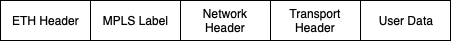
\includegraphics[width=\textwidth]{Final/MPLS.png}
       \caption{MPLS Packet}
       \label{fig:compbest}
\end{figure}


n Normal MPLS Packet, there will be a MPLS Label with bottom-of-stack flag set to 1 pushed on top of the payload. There can be underlying Labels too but with the bottom-of-stack(S) flag set to 
0. The Ethernet header is pushed below all the MPLS Labels and Layer3 Header, Layer 4 header and user data is pushed above all the labels.

\begin{figure}
       \centering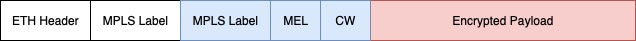
\includegraphics[width=\textwidth]{Final/MPLSOS Packet.jpg}
       \caption{MPLS OS Packet}
       \label{fig:compbest}
\end{figure}


 In the proposed MPLS OS packet, Ethernet Header and top MPLS label remain same. The top MPLS label is then follow another special purpose label with value 15 and bottom-of-stack 0. The special purpose label is then follow MEL followed by CW. Layer3 header, Layer 4 header and user data is encrypted. 

MEL (MPLS Encryption Label) : MEL is like normal MPLS Header, but with the labels from the reserved experimental range (240-255). This label assignment makes it different from normal MPLS Header.Traffic Control (TC) bit is set to the value of the top MPLS Label. S bit is set to 1.

Label 
This label is a special purpose label and so far no special purpose label is allocated by IANA. Hence we have to choose one of the reserved experimental labels from range 240-255.

Traffic Class (TC)
TC is a 3 bit field in the MEL Header. TC is basically used for QoS and ECN. The TC Value should filled the same as the primary outer MPLS Header which is not encrypted.

Bottom of Stack (S)
As MEL is in the bottom of the MPLS Stack, the flag S of the MEL Header should be always set to 1. 

\subsubsection{Control Word (CW)}

\begin{figure}
       \centering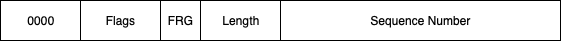
\includegraphics[width=\textwidth]{Final/CW.png}
       \caption{CW Header}
       \label{fig:compbest}
\end{figure}


Control Word (CW) is a 4 byte header. 1st 16 bits of CW is for setting the control word data and the last 16 bits are for sequence number which is nothing but the lower order 16 bits of the nonce. Whenever a packet received at LSR, it will check the underlying protocol of the packet. If the packet is an IP packet, then it will forward by normal routing if so configured. If it is an MPLS packet, it will PUSH/POP the label based on the destination. If the packet have CW and MEL, then the LSR understand that its an encrypted packet and cannot check the underlying protocol for packet forwarding\\

\subsubsection{0000}
The first 4 bits of the CW header is set to 0000 to indicate its a MPLS payload.\\

\subsubsection{Flags} 
Flags is a 4 bit field in the CW Header which contains the session key-id, so that the participants can identify the algorithms and key to be used.\\


\subsubsection{FRG} 
This is a 1 bit field in the CW header and its set to 0 always as MPLS doesn’t support fragmentation\\ 

\subsubsection{Length}
Value of Length should be set to 0 and receiving LSR can ignore this flag.\\

\subsubsection{Sequence Number}
This field contains the low-order 16 bits of the nonce that is currently being used for the agreed encryption parameters. It is indicative of the counter used in the AEAD- AES-GCM encryption which the receiving LSR can use to check it its counter is correct and if it can go ahead with the decryption.\\

Anything from the layer 3 to layer 7 of the packet is encrypted\\

\section{Technologies Involved} 

OpenVswitch, Mininet, OpenFlow, Linux Crypto APIs, Kernel forwarding are the important technologies used in the project. We can see each of them in detail.


\subsection{Mininet} 


Mininet\cite{team}\cite{de2014using} is an emulated network orchestration system. We can emulate Linux hosts, routers, and switches using simple commands and connect them whatever the way and order we want. Mininet links all the emulated hosts and network devices to the same Linux kernel. It is using lightweight virtualisation to make simple and complete network topology which is running the same kernel. The host emulated by Mininet behave exactly the same way the real host behaves except the fact that, there is no real hardware. We can create ssh sessions to all the hosts and switches using the command xterm<space>hostname in the Mininet command line interface.  We can send packets from hosts to host which can be monitored using tcpdump or Wireshark and the packet captured will be absolutely equivalent to the packet captured from a real networking hardware. We can measure speed of the links using tools like Iperf and the link speed between the hosts and routers can be configured or changed using Mininet commands. In short, all the emulated networking devices by Mininet behaves and resembles the same way we expect a hardware product should be behaving.
 
\begin{figure}
       \centering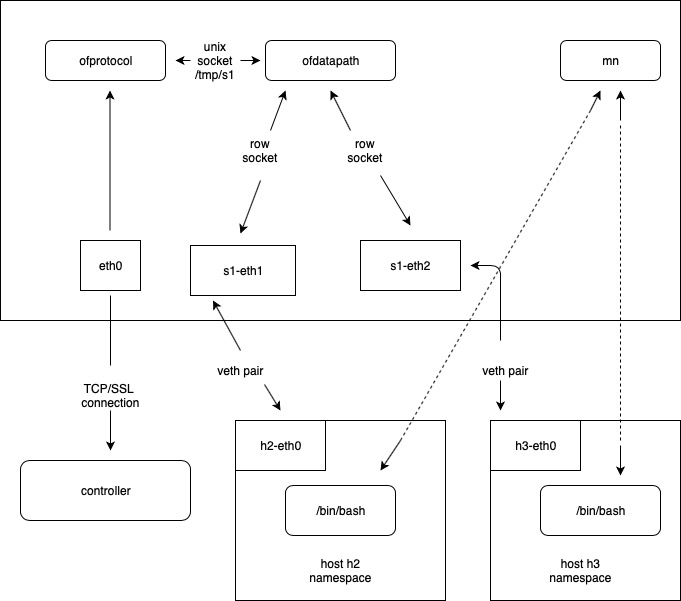
\includegraphics[width=\textwidth]{Final/mininet architecture.jpg}
       \caption{Mininet Architecture}
       \label{fig:compbest}
\end{figure}

\subsection{OpenVSwitch (OVS)} 


OpenVSwitch\cite{openvswitch}\cite{OVS} is an open source multilayer software with Apache 2 license. OpenVSwitch is designed for functioning as a virtual switch in both virtual environment and hardware. The OpenVSwitch code (OVS) can be configured and installed in any linux operating system. It supports most of the linux based virtualization techniques such as Virtual box, KVM, Xen/XenServer etc. The OVS code is written in platform independent C and can be used and ported to other environments. Basically OpenVSwitch is designed for automating large-scale network topology using programmatic extension. OpenVSwitch support standard management interfaces such as Flow, IPFIX, 802.1ag, NetFlow etc. As of now OpenVSwitch cannot run on hypervisors like VMware ESXi and Microsoft Hyper-V, but the development is going on to support them in near future. The 2 major components of OpenVSwitch are  ovs-vswitchd and datapath kernel module. ovs-vswitchd is a daemon which is running in the userspace. Then ovs-vswitchd will not be the same in each operating system but identical in the service. The datapath kernel module functions in the kernel level. The best part is that, we can modify the datapath kernel module and compile and load on the operating system kernel without changing the operating systems kernel. \\

\begin{figure}
       \centering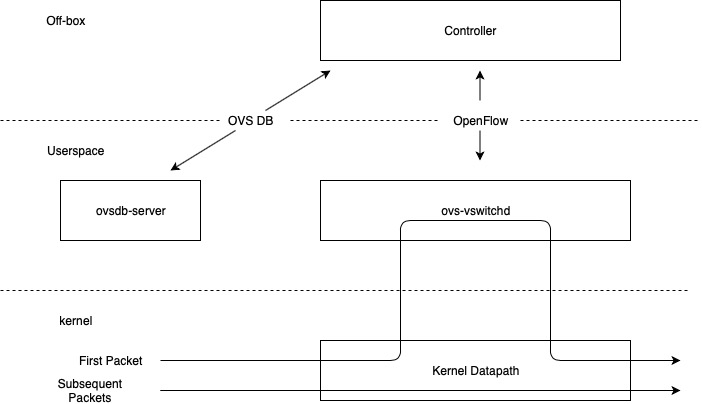
\includegraphics[width=\textwidth]{Final/OVS Architecture-2.jpg}
       \caption{OVS Architecture}
       \label{fig:compbest}
\end{figure}

The first packet entering the NIC is taken into the datapath kernel module and there are 2 possible actions to perform on the packet. If there is any set of actions and logic instructed by the ovs-vswitchd, then perform the logic and forward the packet. If there is no logic instructed, then pass the packet to ovs-vswitchd and wait for the instruction. The subsequent packets belongs to the same flow will be forwarded using the flow logic applied to the first packet.



\subsubsection{Kernel Forwarding} 

All the packets from NIC is taken into the kernel. The daemon ovs-vswitchd is the one instruct the kernel what actions need to be performed on the packet. The actions can be encapsulation, decapsulation, reroute, sampling, drop etc. The kernel datapath will perform these actions on the packet and forward the packets. Generally the ovs-vswitchd actions are instrucrted by the user (administrator) based on the flow. Flow is nothing but packets with same source address, same destination address, same source port, same destination port and same protocol. OVS Actions can be applied even the flows are partially matching. Once the first packet forwarded out with the logic/action from the ovs-vswitchd, the kernel datapath will store the instructions in its local cache and perform the same action if the subsequent packets are eligible for the same actions. If the new packet doesn’t match with the flow marked in the cache, it will treat like the first packet and taken into Userpace and then ovs-vswitchd.


\subsubsection{Userspace Forwarding} 

As we seen in the kernel forwarding, kernel datapath maintain the local cache with the instructions received from ovs-vswitchd for the flows which kernel forwarded to  ovs-vswitchd. If there is no cache available for the incoming flow, then the packet will be taken into ovs-vswitchd which is running in userspace. OpenVSwitch maintain a flow table which is generated based on the cache and this table will say what actions to be performed on the packet. As OpenVSwitch used as SDN switch, the OVS controller and OVS Switch talk to each other using OpenFlow. The user can instruct the OVS controller the actions to be performed in each switch then  OVS Controller instruct the  ovs-vswitchd and finally ovs-vswitchd instructs the datapath kernel module. 

 
\subsection{OpenFlow} 

OpenFLow\cite{2016} is a protocol used for communicating between SDN controller and SDN Switches. As we know that the control plane of the SND Lies in the controller and the controller instruct the data planes (Switches and Routers) what are the actions need to be performed on the incoming packet. This control message exchange between SDN Controller and other nodes usually using open flow protocol. OpenFlow is more like an instruction set similar to x86 instruction set and it provides an open interface to the nodes such as routers and switches. The SDN nodes will have flow tables which is about what are the actions to be performed to an incoming traffic from a particular interface with a particular flow. The open protocol of  OpenFLow is used to program the flow table. The instructions are in the form of flow entries in the flow table. As the SDN controller is remotely accessible from remote locations, researchers and administrators can use open flow to control open flow tables of connected switches and routers and thus control the packet forwarding. \\
 
\subsection{Architecture of Experiment}

The Network topology is emulated using Mininet and packets are processed using openvswitch. the emulated switches will be running with OVSK. Openvswitch can be used in docker and containers too but each docker will have its own overhead and it will affect the network performance. Mininet is very fast to build up the network and tear down the network and hence Mininet is the best choice to demonstrate the MPLS OS using OVS. By default OpenVSwitch will be installed along with Mininet and the Installed openvswitch will be replaced by the modified OpenVSwitch separately installed. Mininet require a controller, a kernel and \\

\begin{figure}
       \centering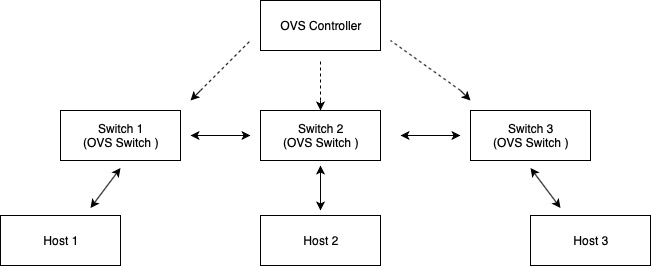
\includegraphics[width=\textwidth]{Final/Experiment Topology.jpg}
       \caption{Experiment Topology}
       \label{fig:compbest}
\end{figure}

In the experiment topology, we will be creating 3 switches (S1, S2 and S3) connected linearly. Each switch is connected 1 host. Switch S1 have 2 interfaces s1-eth1 and s1-eth2. S1-eth1 is connected to Host 1 and s1-eth2 is connected to s2-eth2 of Switch S2. S2-eth1 of switch S2 is connected to Host 2 and s2-eth3 is connected to s3-eth2 of Switch S3. Interface s3-eth1 of S3 is connected to Host 3.
The controller is connected to all the switches and it will update the flow rules in all the switches.\\

The hop by hop behaviour of normal MPLS traffic in our test topology without MPLS OS is as follows:\\

Step 1 : Host 1 initiated an ICMP Ping to Host H3\\
Step 2:  H1 check in its arp table for a the destination MAC address.\\
Step 3: As its the first packet and there is no arp entries for the corresponding destination (Host 3), Host 1 will send an arp request to Host 3.\\
Step 4: Arp request packet will reach Switch 1 ethernet 1 interface and Switch 1 will send the packet out of ethernet 2 interface.\\
Step 5: Arp request packet will reach Switch 2 ethernet 2 interface and Switch 2 will send the packet out of ethernet 3 interface.\\
Step 6: Arp request packet will reach Switch 3 ethernet 2 interface and Switch 3 will send the packet out of ethernet 1 interface.\\
Step 7: H3 will receive the Arp request packet and respond by an ARP reply and it will take the reverse path of ARP Request.\\
Step 8: H1 will send the ICMP packet to the S1 through ethernet 1 ethernet interface.\\
Step 9: S1 will receive the ICMP packet from ethernet 1 interface. S1 will push the MPLS label send out of ethernet 2 interface.\\
Step 10: Switch 2 receive the MPLS packet from ethernet 2 interface and it will send the packet out of ethernet 3 interface.\\
Step 11: Switch 3 receive the MPLS packet from ethernet 2 interface and it will pop the MPLS Label out and send the ICMP packet out of ethernet 1 interface.\\
Step 12:  H3 will receive the ICMP packet from ethernet 1 interface and it will reply back to H1. The reply packet will take the reverse path of incoming ICMP packet, S3 will push the label and S1 will pop the label.\\

The hop by hop behaviour of normal MPLS traffic in our test topology with MPLS OS is as follows:\\

Step 1 : Host 1 initiated an ICMP Ping to Host H3\\
Step 2:  H1 check in its arp table for a the destination MAC address.\\
Step 3: As its the first packet and there is no arp entries for the corresponding destination (Host 3), Host 1 will send an arp request to Host 3.\\
Step 4: Arp request packet will reach Switch 1 ethernet 1 interface and Switch 1 will send the packet out of ethernet 2 interface.\\
Step 5: Arp request packet will reach Switch 2 ethernet 2 interface and Switch 2 will send the packet out of ethernet 3 interface.\\
Step 6: Arp request packet will reach Switch 3 ethernet 2 interface and Switch 3 will send the packet out of ethernet 1 interface.\\
Step 7: H3 will receive the Arp request packet and respond by an ARP reply and it will take the reverse path of ARP Request.\\
Step 8: H1 will send the ICMP packet to the S1 through ethernet 1 ethernet interface.\\

Step 9: S1 will receive the ICMP packet from ethernet 1 interface. S1 will check for the generated shared secret key for encryption.\\
Step 10:As there on key available, S1 will initiate a DH key exchange with S3. S1 will use the incoming ICMP traffic for the DH exchange. S1 will push the MPLS Label and add the MPLS TLV          between MAC header and MPLS header. This TLV will have the information such as DH group, Encryption algorithm, DH Key etc.\\
Step 11: Switch 2 receive the MPLS packet from ethernet 2 interface and it will send the packet out of ethernet 3 interface.\\
Step 12: Switch 3 receive the MPLS packet from ethernet 2 interface and it will pop the MPLS Label and MPLS TLV out and send the ICMP packet out of ethernet 1 interface.Switch 3 will get the DH Key of the S1 from the TLV and it will calculate the shared secret key for encryption and decryption.\\
Step 13: H3 will reply to the ICMP request and the request will reach Switch 3 ethernet 1.\\
Step 14: S3 will push the MPLS Label and add the MPLS TLV between MAC header and MPLS header. This packet will follow the reverse path of packet from H1 to H3.\\
Step 15: When the reverse packet arrived at S1, it will pop the MPLS Label and the MPLS TLV and the send the plain ICMP too H1.\\
Step 16: Switch S1 will get the DH Key of the S3 from the TLV and it will calculate the shared secret key for encryption and decryption.\\
Step 17: Second ICMP Ping packet from H1 to H3 arrived at S1 at ethernet 1 interface.\\
Step 18: S1 will encrypt the payload using  AES-GCM encryption algorithm and the key used is generated in the previous steps. After encryption, a CW header will be pushed on top, then the MPLS Encryption label will be pushed on top. The normal MPLS Header will be pushed on top of the MEL and will send the packet out of ethernet 2 interface.\\
Step 19: Switch 2 receive the MPLS packet from ethernet 2 interface and it will send the packet out of ethernet 3 interface.\\
Step 20: Switch 3 receive the encrypted MPLS packet. It will pop the MPLS label, MEL label and CW header. S3 then decrypt the packet and send then plain ICMP Packet out of ethernet 1 to H3.\\
Step 21: ICMP reply from H3 to H1 will be encrypted at S3 and add MEL, CW Header and MPLS label and send to S1 and S1 will decrypt the packet and send to H1.\\

The Diffie-Hellman Key exchange is not fully integrated in this project work even though the participating switches are exchanging keys and generating shared secret. The MPLS TLV is not exactly same as the specifications since some fields in the TLV such as LSP ID is not available OVS as the labels are manually supplied .HKDF is not implemented in this project and The DH Key is send as an integer decimal in the TLV instead of string. The Generated shared key is used for encryption and decryption.  




%   \chapter{Experiment}
In the last chapter we discussed about the design of MPLS Opportunistic Security. In this chapter I will be explaining the implementation of MPLS OS in the OpenVSwitch Kernel

\section{Infrastructure setup}

The project is implemented in OpenVSwitch kernel. OpenVSwitch is a linux open flow technology which can be installed in Linux machines. All flavours of Linux are supported with OpenVSwitch.\\  

In order to emulate the MPLS Switches and Hosts, either we can install containers in the Linux. Each container can act as an OpenVswitch. Interconnect 2 containers as 2 LSRs connected each other.\\ 

There is an additional overhead when we use multiple containers in the same Linux machine as the kernel crashed many times and the latency collected during the test was unreliable. Hence the implementation further conducted in mininet.\\ 

The topology diagram is given in the figure 3.1. The testing of the final implementation is carried out by sending an icmp ping packet from Host H1 to Host H3.
\subsection{Setting up Mininet}

Mininet can be downloaded and installed in using the command sudo apt-get install mininet. This will install both mininet and openvswitch. The problem is we cannot edit the openvswitch kernel (OVSK) of the openvswitch installed along with the openvswitch. 

To check the working of mininet, we can setup a simple topology of 1 switch and 2 host and ping from both the host using the command sudo mn --test pingall. 

To setup the topology of our experiment, we can use the command sudo mn –topo=linear,3 –switch=ovsk –controller=ovsc 

 
This will initiate 3 switches with one host on each and the switches will be connected serially as shown in the figure 3.1. 

The parameters in the mininet initiation command is given below. 

topo=linear,3: This is for initiating 3 switches with 1 host each and connect the switches linearly. 

–switch=ovsk: This is for using openvswitch kernel as the switch kernel 

–controller=ovsc: This is for choosing openvswitch controller as the openflow SDN controller. 
\subsection{Setting up OpenVswitch}

Installing mininet will install OpenVswitch too. However we cannot edit the kernel of the openvswitch installed along with mininet. We have to install OpenVswitch with version of our choice and then replace the openvswitch installed by mininet from the kernel. 

We can see the module informsation using the command lsmod in the linux.  

We can download the Openvswitch using git clone. The link for downloading is  

git clone https://github.com/openvswitch/ovs.git. Once downloaded we have to bootstrap the image using the script boot.sh in the package and after that we have to configure it using the script configure. Inorder to build the package we have to run the following commands, 



\subsubsection{make} 
\subsubsection{make install}
\subsubsection{make modules_install"}
\subsubsection{/sbin/modprobe openvswitch}\\



Inorder to start the openvswitch, use the following commands,\\

\subsubsection{export PATH=$PATH:/usr/local/share/openvswitch/scripts} 

\subsubsection{ovs-ctl start} 

 \section{Testing the MPLS System}
 
 \subsection{Addition of the MPLS flows}

In order to test the working of MPLS, we have to add MPLS flows to the openvwitch. The topology can be initiated using the command\\ sudo mn –topo=linear,3 –switch=ovsk –controller=ovsc. 

Once the topology is initiated, we can add mpls flows to each OVS Switch using the commands given below. \\

To install mpls flow from S1 to S3 through S2 \\

sudo ovs-ofctl -O OpenFlow13 add-flow s1 "table=0,in_port=1,eth_type=0x800,actions=goto_table:1" 

sudo ovs-ofctl -O OpenFlow13 add-flow s1 "table=1,in_port=1,eth_type=0x800,actions=push_mpls:0x8847,set_field:12->mpls_label,output:2" 

sudo ovs-ofctl -O OpenFlow13 add-flow s2 "table=0,in_port=2,eth_type=0x8847,actions=output:3" 

sudo ovs-ofctl -O OpenFlow13 add-flow s3 "table=0,in_port=2,eth_type=0x8847,actions=goto_table:1" 

sudo ovs-ofctl -O OpenFlow13 add-flow s3 "table=1,in_port=2,eth_type=0x8847,mpls_bos=1,actions=pop_mpls:0x800,output:1" \\

When a packet come from H1 to S1, it will change the Ethernet type to 0x8847. There is another action installed in S1 is that whenever a packet received with type 0x8847, push a MPLS label and then send to S2. In S2 it will simply forward the packet to S3. When a 0x8847 packet come to S3, it will pop the MPLS label and change the Ethernet type to 0x8000 (Normal IP Packet)\\

For the reverse flow from S3 to S1 through S2 \\

sudo ovs-ofctl -O OpenFlow13 add-flow s3 "table=0,in_port=1,eth_type=0x800,actions=goto_table:1" 

sudo ovs-ofctl -O OpenFlow13 add-flow s3 "table=1,in_port=1,eth_type=0x800,actions=push_mpls:0x8847,set_field:32->mpls_label,output:2" 

sudo ovs-ofctl -O OpenFlow13 add-flow s2 "table=0,in_port=3,eth_type=0x8847,actions=output:2" 

sudo ovs-ofctl -O OpenFlow13 add-flow s1 "table=0,in_port=2,eth_type=0x8847,actions=goto_table:1" 

sudo ovs-ofctl -O OpenFlow13 add-flow s1 "table=1,in_port=2,eth_type=0x8847,mpls_bos=1,actions=pop_mpls:0x800,output:1"\\


Here the reverse operation will take place from S3 to S1\\

To install ARP flows from S1 to S3 and reverse\\

sudo ovs-ofctl -O OpenFlow13 add-flow s1 "table=0,in_port=1,eth_type=0x806,actions=output:2" 

sudo ovs-ofctl -O OpenFlow13 add-flow s1 "table=0,in_port=2,eth_type=0x806,actions=output:1" 

sudo ovs-ofctl -O OpenFlow13 add-flow s2 "table=0,in_port=2,eth_type=0x806,actions=output:3" 

sudo ovs-ofctl -O OpenFlow13 add-flow s2 "table=0,in_port=3,eth_type=0x806,actions=output:2" 

sudo ovs-ofctl -O OpenFlow13 add-flow s3 "table=0,in_port=1,eth_type=0x806,actions=output:2" 

sudo ovs-ofctl -O OpenFlow13 add-flow s3 "table=0,in_port=2,eth_type=0x806,actions=output:1" 

 
\subsection{Testing Communication for MPLS}


In order to check the MPLS communication, the Host h1 can initiate a icmp ping to the host h3. We can capture the packets from S1, S2 or S3 and its better to take the packets from S3. If we monitor both the interfaces of S3, one which connected S2 and another connected to H3, we can see that S3 is receiving MPLS packet from S2 and sending as IP packet to H3. 

\section{Implementation of Opportunistic Security in MPLS}


In this section I am going to explain the implementation steps of MPLS OS. The topology I chose the the same as above with 3 switches names S1, S2 and S3 connected serially. For the convenience, I chose S1 as the LSR1 and S3 as LSR3. All the encryption and decryption operations are performed between LSR1 and LSR3. Whenever an ICMP packet come to S1 then it will send the packet to S3 with a MPLS TLV adding a diffie-hellman public key and S3 will generate a shared key. The reverse packet from S3 to S1 will have the TLV from S3 adding its diffie-hellman public key and S1 will generate its shared secret. Further encryption and decryption will be performed with this shared key. For the sake of easy development, I used ICMP packets in clear text for the key management. Once the key is available, all the packets will be sending as ciphertext. The encryption and decryption steps are explained below.  

\subsection{Key Management}

The Key used for encryption and Decryption is derived out of Diffie Hellman Key exchange. There were some challenges while implementing the Key exchange such as finding the power of a large number was giving me zero as the out put. I could not investigate this issue due to time constrains and i had to use small prime number in the code. There are no maths libraries in the Linux kernel and i had to add my own functions instead. Hence i would like to say the key exchange used is a miniature version and there is a scope of improvement. I could not add the GAL which is a new MPLS Label since OVS cannot support multiple labels. few fields in the TLV are not filled such as MPLS Lsp ID, time stamp etc due to the limitations in the OVS. The other challege was when i append all the headers for the key exchange such as Associated Channel Header, Associated Channel TLV, MPLS TLV etc, then wireshark cannot identify the headers and if i send the MPLS TLV alone, then wireshark detects it as Associated Channel Header. Hence debugging with wireshark was a challenge.


\subsection{Changes at S1 (Ingress Switch)}


When a ingress packet comes to S1, it will check for the encryption and decryption keys. If Key are not available, it will initiate a DH key exchange as explained above. Once the key is generated, the payload will be encrypted and a Pseudo Wire Code Word (PWCW) will pushed to the data followed by MEL (MPLS Encryption Label). The encryption is performed by Linux Crypto API and with algorithm AES-128-GCM. Any changes and manipulations to the packet is performed by various operations of SKB Data Structure.\\

\begin{figure}
       \centering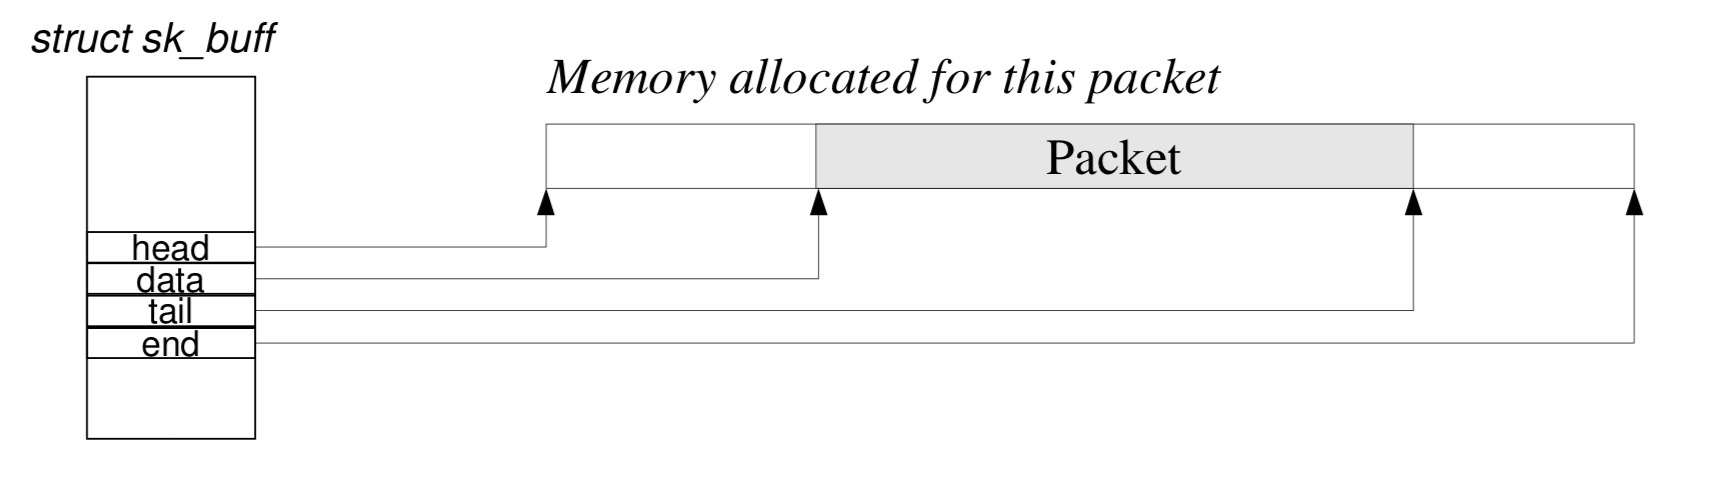
\includegraphics[width=\textwidth]{Final/skbuff.png}
       \caption{SKB Data Structure}
       \label{fig:compbest}
\end{figure}

\subsubsection{Inserting the CW Header}
The steps to add the CW header to the packet is given below.  
The commands given in the table 3.1 are various SKB operations\cite{skbuff2} used for adding a Header and the same is followed for adding CW Header

\begin{table}[htbp]
  \centering
  \caption{skbuff commands}
    \begin{tabular}{|l|p{23.39em}|}
    \toprule
    \hline
    \multicolumn{1}{|c|}{Command} & \multicolumn{1}{c|}{Action} \\
    \midrule
    \hline
    skb\_cow\_head & This command will check if there is enough headroom available in the size of max header length of CW Header \\
    \midrule
    \hline
    skb\_push & This command is used for allocating the header length space for the data structure \\
    \midrule
    \hline
    memmove & This command is used for moving the mac header to the newly allocated space so that we can insert the CW header in the place of MAC header (Between the payload and MAC header) \\
    \midrule
    \hline
    skb\_reset\_mac\_header & This command will reset the pointer to the mac header to the new location of MAC header \\
    \midrule
    \hline
    skb\_mac\_header(skb) + skb->mac\_len & This command points to the start of CW space so that the CV values can be added \\
    \hline
    \bottomrule
    \end{tabular}%
  \label{tab:addlabel}%
\end{table}%



\subsubsection{Encryption of Data}  

Encryption of data is performed by Linux Crypto API and it’s has rich set of all the cryptographic algorithms. For the best understanding of the usage of Linux Crypto APIs, we have to study a bit about the architecture specifications and functional flow of these Crypto APIs \\

There are 2 major components in the Kernel Crypto API which are called Cipher Handles and Request Handles. The Cipher Handles contains all the configurations and settings of the given type of encryption to be used and the request handler handles the encryption requests. \\

The steps to encrypt the packet are given in the Table 3.2,\\


\begin{table}[ht]
  \centering
  \caption{Linux Crypto Commands for encryption}
    \begin{tabular}{|l|l|}
    \toprule
    \hline
    \multicolumn{1}{|c|}{Command} & \multicolumn{1}{c|}{Action} \\
    \hline
    \midrule
    \multicolumn{1}{|p{15.89em}|}{Initialize ’crypto\_aead’ and ’aead\_request’} & \multicolumn{1}{p{22.5em}|}{This command is used for initialising the AEAD Cipher Handler and Request Handler} \\
    \hline
    \midrule
    crypto\_alloc\_aead & \multicolumn{1}{p{22.5em}|}{This command is used for allocating the AEAD Cipher handler} \\
    \hline
    \midrule
    aead\_request\_alloc & \multicolumn{1}{p{22.5em}|}{This command is used for allocating the AEAD Request handler} \\
    \hline
    \midrule
    aead\_request\_set\_callback & \multicolumn{1}{p{22.5em}|}{This command will set the asynchronous call back function which will be executed upon the successful encryption} \\
    \hline
    \midrule
    crypto\_aead\_setkey & \multicolumn{1}{p{22.5em}|}{This command is to set the encryption key which is already generated in the Cipher Handler} \\
    \hline
    \midrule
    aead\_request\_set\_crypt & \multicolumn{1}{p{22.5em}|}{This command will set the data buffers for the encryption process. The plain text data to be encrypted will be concatenated at the start} \\
    \hline
    \midrule
    aead\_request\_set\_ad & \multicolumn{1}{p{22.5em}|}{This command is used for Generating the authentication tag which is used for authenticating the data at the receiving side} \\
    \hline
    \midrule
    crypto\_aead\_encrypt & This command is to trigger the encryption process \\
    \hline
    \bottomrule
    \end{tabular}%
  \label{tab:addlabel}%
\end{table}%




Once the payload data is encrypted, the MEL will be pushed on top of the packet followed by the special purpose label packet and normal MPLS packet. 

\subsection{Changes at S3 (Egress Switch)}
 

When the encrypted packet arrived at S3, it pops the MPLS label at the top along with the MEL. It will check the nonce value in the CW header, and it will compare against its own counter. If both the nonce are matching, it will start the decryption process otherwise the packet will be discarded.\\

\subsubsection{Decryption of Data using Linux Crypto API}

Decryption of the payload is very similar to the encryption process. The only difference is instead of plain text, the input is cipher text which is a concatenated combination of associated data, authentication tag and the cipher text. The authentication tag is used to authenticate the data post the decryption and if there is an authentication failure, it will alert. The flag in crypto_aead_encrypt function is set to decrypt. The output of decryption will give a concatenated combination of associated data and plain text.\\

 

\subsection{Removal of CW}

Just like we added CW header to the packet by manipulation steps used in skbuff, we can pop the CW header from the packet. The SKBuff steps involved in popping the CW header from the packet is given in the Table 3.3.\\


\begin{table}[ht]
  \centering
  \caption{skbuff commands for popping a header}
    \begin{tabular}{|l|p{22.5em}|}
    \toprule
    \hline
    \multicolumn{1}{|c|}{Command} & \multicolumn{1}{c|}{Action} \\
    \hline
    \midrule
    skb\_postpull\_rcsum & This command is used for recalculating the checksum once then MEL is pulled out of the packet \\
    \hline
    \midrule
    memmove & This command is used for moving the MAC header to the place of CW \\
    \hline
    \midrule
    \_\_skb\_pull & This command will pull the size of CW Header (4 bytes) from the top of the skb data structure \\
    \hline
    \midrule
    skb\_reset\_mac\_header & This command is used shifting the MAC header pointer to the new position of the MAC header \\
    \hline
    \midrule
    skb\_set\_network\_header & This command is used for setting the network header pointer to the position of the new network header \\
    \hline
    \bottomrule
    \end{tabular}%
  \label{tab:addlabel}%
\end{table}%




\section{Testing the MPLS OS System}
Once the Opportunistic Security is implemented in the OVS code, we have to compile the OVS kernel. All the kernel files of the OVS is kept in the folder called datapath and the majority of the changes are performed in the file called action.c. The header files are kept under linux/compat/include/net. The OVS have a makefile which is used for the compilation. Once the compilation is done if we have previously installed OVS in the Linux kernel, we have to remove is by rmmod or modprobe. A simple ’rmmod openvswitch’ will remove the openvswitch from the linux kernel. Make sure to stop the openvswitch before compiling the code. Detailed building, compiling and loading steps of openvswitch is submitted in the git repository of the research report. Once the compilation is done, we can load the openvswith to the linux kernel using modprobe,  ’modprobe openvswitch’. We can check if we correctly loaded the openvswitch in the kernel by using lsmod.

\subsection{Addition of the MPLS OS flows}

The difference between the flows of traditional MPLS and MPLS OS is the addition of Special Purpose Label, the CW and the MEL. These header additions are not performed by the OpenFlow Flow because there is only very limited packet modifications are possible in OpenFlow such as changing the ether type. These headers are added only when a packet is send encrypted which is only happen by end of a successful key exchange between the participating LSRs. As discussed above there are 3 MPLS labels are added in MPLS OS such as the MEL with value 1, the special purpose label with label value 15 and another MPLS label for routing. The issue encountered during the development is that packet was discarded at S3 without sending to the destination host and the reason was the OVS cannot pop multiple labels of the same packet and the OVSK was forwarding the packet to userspace\cite{OVSMail2}E. This issue has to be fixed by OVS and meantime the workaround adapted is that instead of pushing 3 Labels, push a single label with value 1and this label will act as the functional combination of all 3 labels proposed in the design.\\

With the workaround the modified MPLS FLow is as given below,\\

sudo ovs-ofctl -O OpenFlow13 add-flow s1 "table=0,in_port=1,eth_type=0x800,actions=goto_table:1" 

sudo ovs-ofctl -O OpenFlow13 add-flow s1 "table=1,in_port=1,eth_type=0x800,actions=push_mpls:0x8847,set_field:1->mpls_label,output:2" 

sudo ovs-ofctl -O OpenFlow13 add-flow s2 "table=0,in_port=2,eth_type=0x8847,actions=output:3" 

sudo ovs-ofctl -O OpenFlow13 add-flow s3 "table=0,in_port=2,eth_type=0x8847,actions=goto_table:1" 

sudo ovs-ofctl -O OpenFlow13 add-flow s3 "table=1,in_port=2,eth_type=0x8847,mpls_label=1,mpls_bos=1,actions=pop_mpls:0x800,output:1" \\

 

sudo ovs-ofctl -O OpenFlow13 add-flow s3 "table=0,in_port=1,eth_type=0x800,actions=goto_table:1" 

sudo ovs-ofctl -O OpenFlow13 add-flow s3 "table=1,in_port=1,eth_type=0x800,actions=push_mpls:0x8847,set_field:1->mpls_label,output:2" 

sudo ovs-ofctl -O OpenFlow13 add-flow s2 "table=0,in_port=3,eth_type=0x8847,actions=output:2" 

sudo ovs-ofctl -O OpenFlow13 add-flow s1 "table=0,in_port=2,eth_type=0x8847,actions=goto_table:1" 

sudo ovs-ofctl -O OpenFlow13 add-flow s1 "table=1,in_port=2,eth_type=0x8847,mpls_label=1,mpls_bos=1,actions=pop_mpls:0x800,output:1" \\

 

sudo ovs-ofctl -O OpenFlow13 add-flow s1 "table=0,in_port=1,eth_type=0x806,actions=output:2" 

sudo ovs-ofctl -O OpenFlow13 add-flow s1 "table=0,in_port=2,eth_type=0x806,actions=output:1" 

sudo ovs-ofctl -O OpenFlow13 add-flow s2 "table=0,in_port=2,eth_type=0x806,actions=output:3" 

sudo ovs-ofctl -O OpenFlow13 add-flow s2 "table=0,in_port=3,eth_type=0x806,actions=output:2" 

sudo ovs-ofctl -O OpenFlow13 add-flow s3 "table=0,in_port=1,eth_type=0x806,actions=output:2" 

sudo ovs-ofctl -O OpenFlow13 add-flow s3 "table=0,in_port=2,eth_type=0x806,actions=output:1" 

\subsection{Testing Communication for MPLS with OS}

MPLSOS works very similar to traditional MPLS. The difference is that the packets between 2 participating LSRs are encrypted.The key for encryption and decryption is generated after a DH Key exchange. The very first packet send between 2 participating LSRs (S1 and S3 in the experiment setup) is a DH Key exchange which is in plain text and there will be an MPLS TLV\cite{__2017}\cite{__2014}\cite{___2009} between the MPLS header and Ethernet Header.

\begin{figure}[ht]
       \centering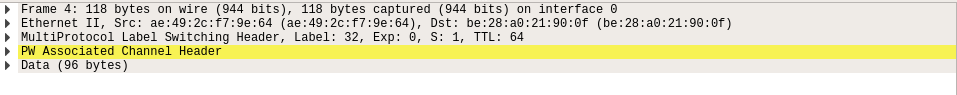
\includegraphics[width=\textwidth]{Final/MPLS_TLV.png}
       \caption{MPLS TLV}
       \label{fig:compbest}
\end{figure}

This TLV will have the DH Group, DH Key, Encryption Algorithm etc and the receiving LSR can calculate the shared secret key for encryption and decryption.\\

Once the key is generated, the very packet onwards the LSR will start encrypting using the key generated. In the experiment setup the host H1 will send plaintext ICMP Ping to Host H3. The packet will arrive Switch S1 which is a participating LSR and S1 encrypt the packet, then add MEL and CW, then send to S3 through S2. S3 will pop the MEL and CW, then decrypt the packet and forward the plain ICMP packet to H3. ICMP Reply from H3 to H1 will follow the reverse path of the request packet.


\begin{figure}[ht]
       \centering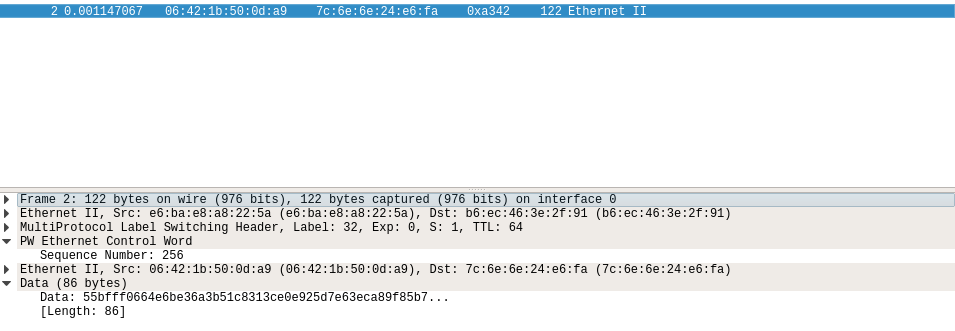
\includegraphics[width=\textwidth]{Final/MPLSOS_Working.png}
       \caption{MPLSOS Packet}
       \label{fig:compbest}
\end{figure}

%   \chapter{Performance Evaluation of MPLS OS }
We know that packet encryption and decryption definitely impact the performance of the network especially in the form of throughput reduction, increased latency, reduced Scalability etc. In order to publish a proof of concept document with impact of MPLS OS in the network, a study with comparing the network performance with and without MPLS OS is required. A test with RFC2544 is best to tell the network performance. Network throughput UDP and TCP with different payload size and mixed size is required so that we can understand how the system is behaving with different type of packets. There are many tools available to perform performance testing of a real hardware networking equipment. However the experimental setup is a Linux machine with emulated hosts and switches using Mininet, hence the external testing tools cannot be used. The future development plan is to bring up the OVS with MPLS OS in a bare metal switch which will be ideal to perform all the performance testing with external tools and document a comprehensive report. I had an attempt to test network throughout of emulated experiment setup using Iperf but, the Kernel of the PC Crashed during the test and could not measure the throughput and I had to reboot the system and give up the attempt. Finally I limited with calculating Latency using Routing Trip Time of ICMP Ping packets.

\subsection{Round Trip Time Calculation (RTT)}

Latency is the term used to define the time difference between a packet transmission and reception, in other words delay in the network. There are tools which time stamp the packet before sending and at the reception, they can compare the timestamp of the packet with the local time of the receiving device and calculate the latency. The issue here is the time synchronisation, sometimes the clock of the transmitting device and the receiving device are follow different clock. We can use same NTP Server in both sender and receiver to avoid the clock miss match. Time stamping a packet need external tools and hence I cannot perform the real latency test and restricted with Round Trip Time calculation of ICMP Ping packets. Round Trip Time is the time the packet took to travel from Host A to Host B and then return to Host A. This is not a real latency test because the latency should be calculated from the delay the packet experienced when leaving the Host A and Arriving at Host B. But still RTT will give some ideas about the delay in the overall network. The number of Hopes will influence the RTT as each hope as to process the packet by changing the address and TTL field and its always good to test RTT between 2 directly connected layer 3 machines.\\

In my study, I performed RTT for a sequence of 100 packets with MPLS Opportunistic Security and without Opportunistic Security. I could see that RTT of MPLS OS packet is almost double normal MPLS packet and it was very much expected since encryption, decryption and encapsulation, decapsulation for sure cause delay. As we know that there will be slight difference in the latency when the packet size changes and keeping this in mind I performed 2 different test such as RTT with small packets and RTT with Large packets.\\

\begin{figure}
       \centering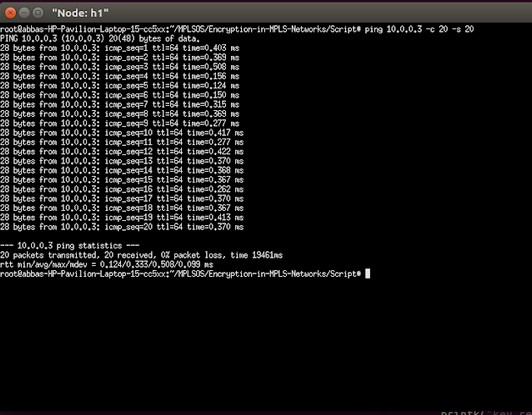
\includegraphics[width=\textwidth]{Final/MPLSOS_Small.jpg}
       \caption{MPLSOS RTT test with small packets}
       \label{fig:compbest}
\end{figure}

\begin{figure}
       \centering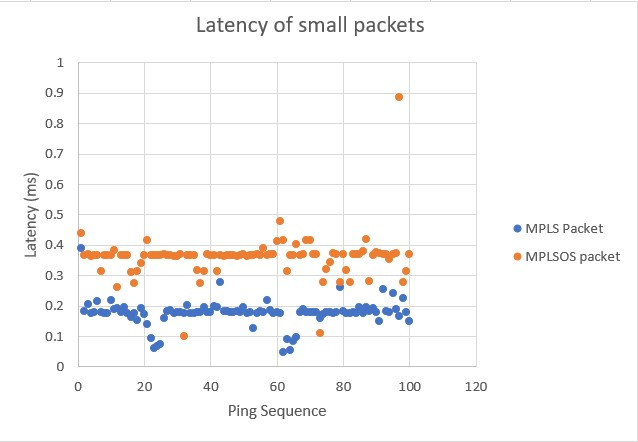
\includegraphics[width=\textwidth]{Final/Latency_small.jpg}
       \caption{RTT comparison of small packets}
       \label{fig:compbest}
\end{figure}


Figure 4.2 shows the RTT comparison of small packets with a minimum payload. The blue dots represents latency of normal MPLS packets and orange dots represents MPLS OS packets.
From Figure 4.1 and 4.2, We can see that the average RTT of normal MPLS packets are just below 0.2 ms and that of MPLS OS packets are just below 0.4 ms which is almost double to the first one.\\


\begin{figure}
       \centering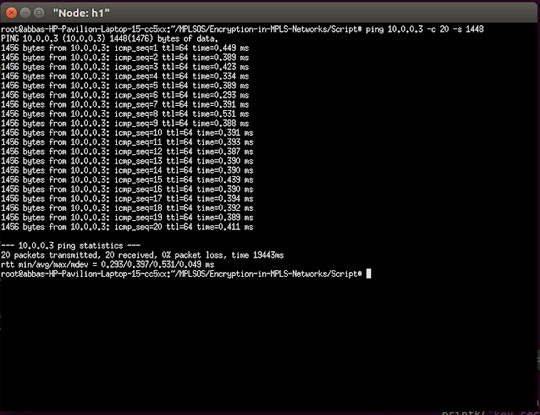
\includegraphics[width=\textwidth]{Final/MPLSOS_Large.jpg}
       \caption{MPLSOS RTT test with large packets}
       \label{fig:compbest}
\end{figure}

\begin{figure}
       \centering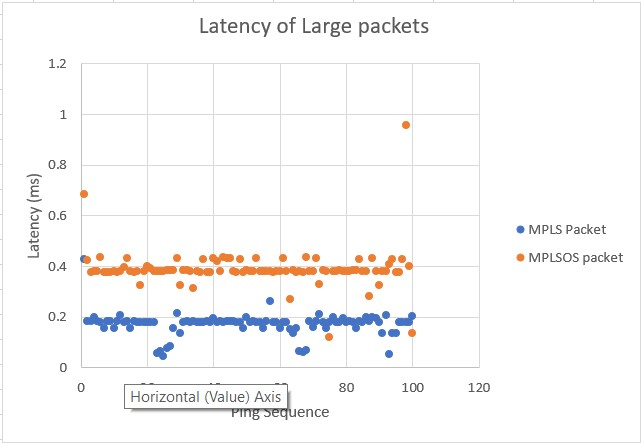
\includegraphics[width=\textwidth]{Final/Latency_large.jpg}
       \caption{RTT comparison of large packets}
       \label{fig:compbest}
\end{figure}


Figure 4.4 shows the latency comparison of Large packets with and without MPLS OS. The packets in the wire was exactly 1514 which is the MTU. Surprisingly the latency of large packets was very similar to small packets and I believe this is because of the emulation environment and behaviour will be different in the real hardware case.\\

\begin{figure}
       \centering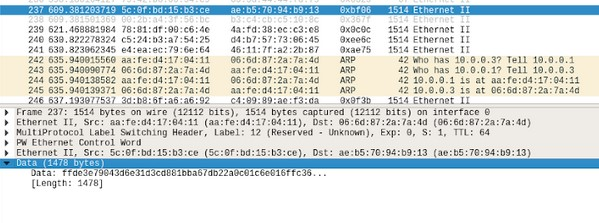
\includegraphics[width=\textwidth]{Final/mplsos_1514.jpg}
       \caption{1514 bytes MPLSOS Packet}
       \label{fig:compbest}
\end{figure}

Finally my finding is that there will be almost 50 percent performance reduction if we use MPLS OS between 2 adjacent LSRs(Hope by Hope) and the performance degradation will be less when we use MPLS OS as an end to end solution in a large MPLS Cloud. To get the exact figure of performance degradation, a real hardware deployment and testing of MPLS OS is required.\\

\subsection{MTU Limitation}

We know that unlike IP Packets, MPLS packet doesn’t undergo IP Fragmentation if the packet size exceeds the MTU. MTU is the maximum size of the frame the layer 2 can accept and the packet is consisting of payload and headers. If we use MPLS, it will add 4 bytes to the frame per labels pushed. If we push 2 labels, it will add 8 bytes. In MPLS OS, we add a CW Header which 4 bytes in size and a 4 bytes header MEL apart from the label. The cipher text (encrypted payload) of MPLS OS larger than plain text payload. So the packet going out of an MPLS OS Router will be much larger than the incoming packet and much care should be given here to make sure that overall packet size shouldn’t exceed the MTU. I kept the MTU of the experiment setup as 1514 byes and I tested a packet with 1515 bytes and the result was the packet got dropped by the LSR which was expected. \\


\begin{figure}
       \centering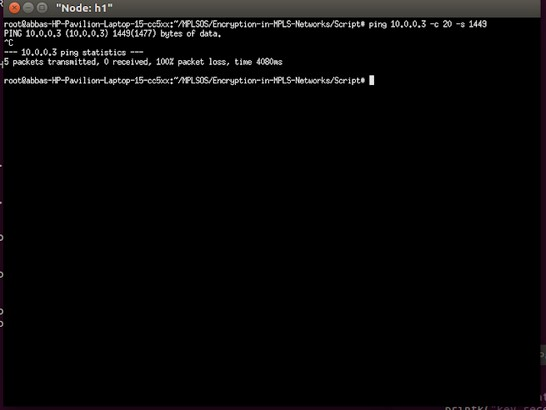
\includegraphics[width=\textwidth]{Final/MPLS_Frag.jpg}
       \caption{1515 bytes MPLSOS Packet}
       \label{fig:compbest}
\end{figure}
%   \chapter{Future Work}
\section{Enhancement of Key Exchange}

I have added DH Key exchange in this project, however, the implementation is not complete. since the experiment is performed in Openvswitch, the labels are manually populated and there is no LSP as such to populate in the MPLS TLV. The same plain text packet from the host H1 to host H3 is used for exchanging the TLV and due to lack of available APIs and time, could not implement HKDF for Key expansion. I tried to Initiate a new packet from the kernel between the participating LSRs for key management but the Linux kernel doesnt have the headers required for creating the MPLS TLV, but its easily addable in the OVS Kernel, and that's why I used the ping packet for exchanging the TLV. I will address these issues in the next phase of the development. The key focus in the next phase with respect to Key management are 1) Use a kernel generated packet between LSRs, 2) Fill the MPLS TLV with all the required fields including LSP ID, 3) Use HKDF for Key expansion.



\section{Implementation on a real hardware}
As we saw in the last chapter, evaluating the performance of MPLS OS is not easy. The results of the virtual system may not follow that of a real hardware. In the results section we saw that packet size didn't affect much in terms of latency, but that won't be the case of a hardware based switch. Once the feature is implemented on a real switch, it will give the provision to test the performance with traffic originated from out side. 


\section{Performance Evaluation using External Traffic}

I had an attempt to measure throughput using Iperf but had to give up the attempt as the kernel was crashing the moment i Initiated the traffic and this is a limitation in virtual environment. Once the feature is implemented on a real hardware, then we can test the feature using external traffic. The real switches have traffic ports which can be connected to traffic tools such as IXIA, Spirent etc. Tests like RFC2544 and Scalability will give a complete picture of robustness of the feature. In the next phase i will be conducting a thorough performance evaluation and document the results.





%\begin{thebibliography}{refs}                   %% Start your bibliography here; you can
\bibliographystyle{ieeetr}
\bibliography{refs}                               %% also use the \bibliography command
%\end{thebibliography}                             %% to generate your bibliography.


\addcontentsline {toc}{chapter}{Appendices}       %% Force Appendices to appear in contents
\begin{appendix}
 \chapter*{Appendix}

The OVS codebase and the scripts to bring up the experiment setup are uploaded in the github public repository.

The link is : https://github.com/abbas443/MPLSOS



% \include{appendix2}
\end{appendix}


%\addcontentsline {toc}{chapter}{Bibliography}     %% Force Bibliography to appear in contents


\end{document}                                    %% END THE DOCUMENT
